\documentclass[11pt,letterpaper]{article}
\usepackage[margin=1in,headheight=16pt,footskip=28pt]{geometry}
\usepackage[T1]{fontenc}
\usepackage{libertinus}
\usepackage{microtype}
\usepackage{amsmath,amsthm,mathtools}
\usepackage{booktabs,tabularx,array,enumitem}
\usepackage{tikz}
\usetikzlibrary{arrows.meta,positioning,calc,fit}
\usepackage{fancyhdr,lastpage,needspace,float}
\usepackage{xurl}
\usepackage[hidelinks]{hyperref}
\usepackage{cleveref}
\usepackage{titlesec}
\usepackage{xcolor}
\definecolor{ink}{RGB}{28,28,28}
\definecolor{mute}{RGB}{82,82,82}
\definecolor{pale}{RGB}{247,247,247}
\hypersetup{pdftitle={MUSIC of an Automated Theorem Prover: Possible Dream Families, Realizability Complexes, and Certified Reflection},pdfauthor={Brian Tenneson; AI-assisted exposition},pdfsubject={AMLD+0 dreaming games, powersets, certified search, combinatorial topology},pdfkeywords={automated theorem proving, dreaming, MUSIC, AMLD+0, simplicial complexes, certified reflection}}
\color{ink}
\setlength{\parindent}{1.35em}
\setlength{\parskip}{0.10em}
\setlength{\emergencystretch}{2em}
\linespread{1.035}
\setlist[itemize]{topsep=3pt,itemsep=1pt,leftmargin=1.65em}
\setlist[enumerate]{topsep=3pt,itemsep=2pt,leftmargin=1.9em}
\titleformat{\section}{\Large\bfseries}{\thesection.}{.65em}{}
\titleformat{\subsection}{\large\bfseries}{\thesubsection.}{.65em}{}
\titlespacing*{\section}{0pt}{18pt}{9pt}
\titlespacing*{\subsection}{0pt}{13pt}{5pt}
\pagestyle{fancy}
\fancyhf{}
\fancyhead[L]{\small\textsc{MUSIC of an ATP}}
\fancyhead[R]{\small\textsc{Research exposition / 2026}}
\fancyfoot[C]{\small\thepage\ / \pageref{LastPage}}
\renewcommand{\headrulewidth}{0.3pt}
\newtheorem{theorem}{Theorem}[section]
\newtheorem{proposition}[theorem]{Proposition}
\newtheorem{corollary}[theorem]{Corollary}
\newtheorem{lemma}[theorem]{Lemma}
\theoremstyle{definition}
\newtheorem{definition}[theorem]{Definition}
\newtheorem{example}[theorem]{Example}
\theoremstyle{remark}
\newtheorem{remark}[theorem]{Remark}
\newcommand{\PSet}{\mathcal{P}}
\newcommand{\Dream}{\mathcal{D}}
\newcommand{\Music}{\operatorname{MUSIC}}
\newcommand{\JMusic}{\operatorname{MUSIC}_{\mathrm J}}
\newcommand{\Fin}{\operatorname{Fin}}
\newcommand{\Cn}{\operatorname{Cn}}
\newcommand{\Runs}{\operatorname{Runs}}
\newcommand{\eps}{\varepsilon}
\newcommand{\Def}{\mathrel{\mathop:}=}
\newcommand{\blank}{\varnothing}
\newcommand{\status}[1]{\textsf{#1}}
\newcommand{\citeurl}[1]{\url{#1}}
\begin{document}
\begin{center}
  {\LARGE\bfseries MUSIC of an Automated Theorem Prover\par}
  \vspace{4pt}
  {\large\itshape Possible Dream Families, Realizability Complexes, and Certified Reflection\par}
  \vspace{10pt}
  {\large\textless Brian Tenneson\textgreater\par}
  \vspace{4pt}
  {\small November 3, 2026 \quad $\cdot$ \quad Research article, version 2.0 \quad $\cdot$ \quad AMLD+0 research program\par}
\end{center}
\vspace{3pt}
\begin{center}
\begin{minipage}{.91\textwidth}
\footnotesize\noindent\textbf{AI-authorship and reliability notice.} This article was prepared through human-directed, AI-assisted mathematical exposition. The full authorship and reliability disclaimer, including verification limitations, appears on the final page.
\end{minipage}
\end{center}
\vspace{7pt}
\begin{abstract}
A condition-relative construction called \emph{MUSIC} associates with an automated theorem prover (ATP), its certified BANK, internal dreaming players, and a complete starting or intermediate condition the set of all sets of possible dreams. Each dream is itself a union of location reports generated during a legal generalized-board-game episode. We formalize the literal construction as $\Music(c)=\PSet(\Dream_c)$, distinguishing it from a different object---the family of \emph{jointly realizable} dream collections. We establish exact reconstruction of the possible-dream space from MUSIC, monotonicity and cardinality laws, and a factorization criterion that identifies which history-dependent claims survive report-union abstraction. The finite jointly realizable collections form an abstract simplicial complex, capable of distinguishing systems that have identical MUSIC in the powerset sense. We give finite obstruction examples and distinguish finite from infinite co-realizability. We further prove a verifier-gated conservativity result: use of MUSIC to propose search directions does not alter object-theoretic consequence so long as independently checked admission and dependency scope remain intact. Counterexamples show that unordered reports need not preserve histories, and that a richer possibility space does not imply more theorems, automatic discovery, or lower cost. The paper distinguishes elementary consequences of standard set theory from architecture-specific definitions, provides finite examples and diagrams, and formulates a falsifiable program for certified reflective search. All proofs are mathematical arguments reviewed in this exposition; none is represented as a machine-checked theorem or an observed deployment of AMLD+0.
\end{abstract}
\noindent\textbf{Keywords.} automated theorem proving; AMLD+0; generalized board games; dreaming; BANK; powerset; trace abstraction; simplicial complexes; proof certificates; reflection.

\tableofcontents
\vspace{6pt}
\section{The motivating question}
An ATP has a formal theory and a proof-search procedure. In the dreaming proposal developed in Tenneson's five-ATP federation manuscript \cite{tenneson-dreaming}, individual ATP members may also have internal cooperative processes---among them Knowledge and Awareness, and potentially Intuition and other traits---operating within generalized board games. The activity called a \emph{dream} is meant to explore, reconstruct, or reconsider evidence without giving unverified imagination authority to declare theorems.

The present proposal introduces a distinct mathematical object. Rather than naming an individual melody or one recorded play, \emph{MUSIC} is to be the \emph{set of sets of possible dreams}, relative to the BANK, players, and starting or intermediate condition. A dream is a union of location reports. The word ``possible'' is crucial: MUSIC concerns permitted counterfactual episodes, not just past observations.

Three logically different questions then arise. First, is MUSIC already definable from the existing theory? Second, what facts about MUSIC follow as theorems, as opposed to being stipulated in definitions? Third, can MUSIC inform proof discovery while the certified theory remains sound? Answering them requires separating a mathematical \emph{space of possibilities} from a \emph{proof certificate}. The same distinction governs the BANK/Board architecture in \emph{Who Checks the Federation?}, Integrated Research Edition 7.10 \cite{tenneson-wcf}, and the invariant-core approach \cite{tenneson-core}.

\paragraph{Scope of the settlement.} Our principal settlement is a conditional \status{P} for \emph{set-theoretic definability and the structural claims proved below}. No universal improvement in runtime, proof probability, epistemic capability, or originality is established. This paper is a mathematical extension of a proposed architecture, not an attestation that these operations were implemented by a separately running federation.

\section{A typed mathematical setting}
\begin{definition}[Frozen ATP dreaming condition]
A \emph{condition} is a tuple
\begin{equation}\label{eq:condition}
 c=(A,B,P,s,G,\Lambda,V),
\end{equation}
where $A$ is an ATP; $B$ is its certified BANK and permitted evidence interface; $P=\{p_1,\ldots,p_N\}$ is a fixed finite set of internal game players; $s$ is a \emph{complete} starting or intermediate state; $G$ specifies legal game transitions, scheduling, and permission rules; $\Lambda$ defines location-report formats; and $V$ specifies the independently authorized checking and admission interface. All components are fixed while evaluating the particular condition $c$.
\end{definition}
The full state $s$ is essential. A snapshot showing merely piece locations may omit a clock, whose turn it is, unseen permissions, BANK versions, or pending messages; two such visually identical snapshots can have different legal continuations. A $2$-dimensional infinite board such as $\mathbb Z^2$ is locally finite under its usual adjacency relation, but \emph{local finiteness of board adjacency alone does not determine the branching of the game's legal transition relation}. The latter must be part of $G$.

The number $N$ counts \emph{internal dreaming players}. It is not the number of federation-level ATPs and is not necessarily the number of AMLD+0 specialist roles $\status{P},\status{R},\status{D},\status{I},\status{C}$. This respects the separation of three counts in \cite{tenneson-dreaming}: one federation, five ATP members in that example, and the separate number of internal players hosted by each ATP.

\begin{definition}[Location reports, histories, and dreams]
Choose a set $U_c$ of typed atomic location records. A \emph{location report} is a subset $r\subseteq U_c$; a report may be a singleton containing a record $(\mathrm{episode},\mathrm{turn},\mathrm{player},\mathrm{piece},x,y,\mathrm{tag})$. Let $\mathcal H_c$ be the collection of legal dream episodes reachable from $s$ under $G$. For $h\in\mathcal H_c$, let $R(h)$ be the family of its reports. Define
\begin{equation}\label{eq:dream}
 d(h)\Def \bigcup_{r\in R(h)}r\subseteq U_c.
\end{equation}
Thus a \emph{dream}, by the proposed extensional definition, is the union $d(h)$, not necessarily the full ordered history $h$.
\end{definition}
We require $U_c$ and $\mathcal H_c$ to be sets, with $R$ a set-valued report assignment and $d$ its corresponding function. Alternatively, one may define $\Dream_c$ directly as a subset of $\PSet(U_c)$ by a formula of the ambient set theory with set parameters; this is a \emph{different sufficient formulation}, not an equivalence of assumptions. The definitions thus invoke ordinary Separation and Powerset rather than an unrestricted set of all histories. A history may be finite or infinite if its coded collection is a set; the case studies below use finite episodes. An implementation must retain, within the reports or in an authenticated linked record, every proof-relevant field its later claims require.

\begin{definition}[Possible-dream space and literal MUSIC]\label{def:music}
The possible-dream space at $c$ is
\begin{equation}\label{eq:D}
 \Dream_c\Def \{d(h):h\in\mathcal H_c\}\subseteq\PSet(U_c).
\end{equation}
The proposed \emph{MUSIC of $A$ at condition $c$} is
\begin{equation}\label{eq:music}
 \boxed{\Music(c)\Def\PSet(\Dream_c)=\{X:X\subseteq\Dream_c\}.}
\end{equation}
\end{definition}
The two levels of braces are intentional: $d\subseteq U_c$ is a dream, $X\subseteq\Dream_c$ is a \emph{collection of dreams}, and $\Music(c)$ is the set of all such collections. For example, $\{d_1,d_2\}\in\Music(c)$ whenever each of $d_1$ and $d_2$ is individually possible. It does \emph{not} follow that both can happen in a single execution.

\begin{figure}[H]
\centering
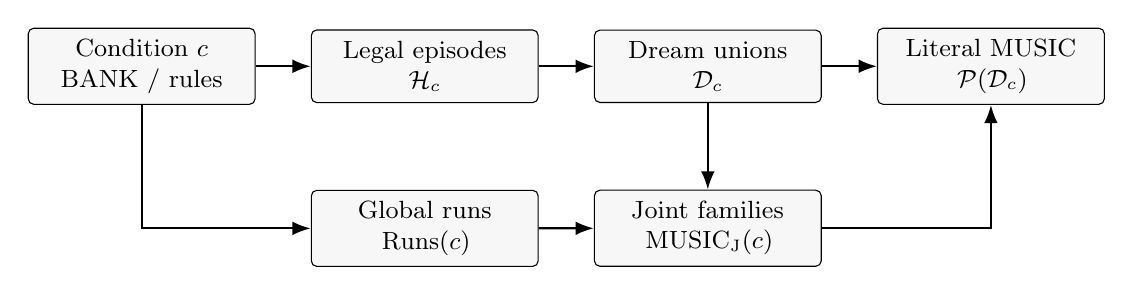
\begin{tikzpicture}[node distance=11mm and 7mm,>=Latex,
every node/.style={font=\small},
box/.style={draw,rounded corners=2pt,align=center,fill=pale,
minimum height=9mm,text width=26mm,inner sep=4pt}]
\node[box] (c) {Condition $c$\\BANK / rules};
\node[box,right=of c] (h) {Legal episodes\\$\mathcal H_c$};
\node[box,right=of h] (d) {Dream unions\\$\Dream_c$};
\node[box,right=of d] (m) {Literal MUSIC\\$\PSet(\Dream_c)$};
\node[box,below=11mm of h] (runs) {Global runs\\$\Runs(c)$};
\node[box,below=11mm of d] (j) {Joint families\\$\JMusic(c)$};
\draw[->,thick] (c) -- (h);
\draw[->,thick] (h) -- (d);
\draw[->,thick] (d) -- (m);
\draw[->,thick] (c.south) |- (runs.west);
\draw[->,thick] (runs) -- (j);
\draw[->,thick] (d) -- (j);
\draw[->,thick] (j.east) -| (m.south);
\end{tikzpicture}
\caption{The arrows indicate definitional dependence and inclusion. Literal MUSIC uses only the possible dream unions; the joint family additionally depends on the occurrence sets of legal global runs. The diagram is conceptual, not an implementation.}
\label{fig:two-musics}
\end{figure}

\section{The elementary theory of literal MUSIC}
The first results are immediate but valuable. They show which properties are \emph{already theorems of powersets}, independent of any special property of ATPs.

\begin{theorem}[Recovery and exact equivalence]\label{thm:recovery}
For any admissible condition $c$,
\begin{equation}\label{eq:recover}
\bigcup\Music(c)=\Dream_c.
\end{equation}
Consequently $\Music(c_1)=\Music(c_2)$ if and only if $\Dream_{c_1}=\Dream_{c_2}$, for conditions whose dreams have been represented in a common report universe or identified by an explicitly declared translation.
\end{theorem}
\begin{proof}
Every member $X$ of $\PSet(\Dream_c)$ is contained in $\Dream_c$, so its union is contained in $\Dream_c$. Conversely, for each $d\in\Dream_c$, the singleton $\{d\}$ belongs to $\PSet(\Dream_c)$, putting $d$ in the union. This argument also holds when $\Dream_c=\blank$. Equal powersets have equal unions; equal underlying sets have equal powersets.
\end{proof}

\begin{definition}[Musical equivalence]
Conditions $c_1,c_2$ are \emph{extensionally musically equivalent}, written $c_1\sim_M c_2$, when $\Music(c_1)=\Music(c_2)$ after any declared representation translation.
\end{definition}
This is an equivalence relation. It does \emph{not} entail equal verification cost, available resources, timing, certificate provenance, local BANK contents, or the same sequences of moves. The theorem says exactly that the \emph{sets of report-union dreams} coincide.

\begin{proposition}[Cardinality and algebra]\label{prop:algebra}
If $|\Dream_c|=m<\infty$, then $|\Music(c)|=2^m$. If $\Dream_c$ is infinite, $|\Music(c)|>|\Dream_c|$. With set union, intersection, and complementation relative to $\Dream_c$, $\Music(c)$ is a complete atomic Boolean algebra (including the degenerate one-element case when $\Dream_c=\blank$).
\end{proposition}
\begin{proof}
There are two independent membership decisions per element of a finite $\Dream_c$. The infinite assertion is Cantor's theorem. Arbitrary unions and intersections of subsets of $\Dream_c$ remain subsets, complementation is taken within $\Dream_c$, and the atoms are its singleton subsets when they exist.
\end{proof}
Thus ten possible distinct dreams imply $2^{10}=1024$ abstract members of MUSIC. This is not a claim that the ATP can enumerate, store, or perform the members. An uncountable powerset may arise even from a countably infinite space of possible dreams.

\begin{proposition}[Monotonicity with its necessary qualification]\label{prop:monotone}
For two conditions represented in the same universe,
\[
\Dream_{c_1}\subseteq\Dream_{c_2}
\quad\Longleftrightarrow\quad
\Music(c_1)\subseteq\Music(c_2).
\]
A larger BANK does \emph{not}, by itself, imply either inclusion.
\end{proposition}
\begin{proof}
The forward implication is monotonicity of powersets. For the converse, if $d\in\Dream_{c_1}$ then $\{d\}\in\Music(c_1)\subseteq\Music(c_2)$, so $d\in\Dream_{c_2}$. To see why mere BANK growth is insufficient, suppose a policy allows a speculative dream before evidence $e$ is accepted but forbids it afterwards. The larger BANK yields fewer legal paths. Under a different policy new evidence might enable additional paths. An inclusion conclusion therefore requires a separate \emph{permissive-extension} or trace-simulation hypothesis.
\end{proof}

\section{Information lost by union and a precise repair}
A union of reports is a set, and sets forget multiplicity and ordering unless these are encoded within their elements. This is not a defect in set theory; it is a design obligation for a representation intended to support historical or proof-relevant inferences.

\begin{example}[Two histories, one untagged dream]\label{ex:collision}
Let reports contain only visited coordinates. On a segment of the infinite grid, two legal episodes visit
\[
 h_1:(0,0)\to(1,0)\to(2,0),
 \qquad
 h_2:(0,0)\to(1,0)\to(0,0)\to(1,0)\to(2,0).
\]
Both report unions are $\{(0,0),(1,0),(2,0)\}$, despite unequal lengths and different sequences. Hence $d(h_1)=d(h_2)$ and no inverse map on such dream sets can reconstruct both histories.
\end{example}

\begin{definition}[Observation map and invariant]\label{def:factor}
Write $q:\mathcal H_c\to\Dream_c$ for $q(h)=d(h)$. A \emph{history property} is a map $f:\mathcal H_c\to Y$ into a declared set $Y$ (for instance, a verified-evidence type, charged cost, or terminal result). We say $f$ is \emph{MUSIC-recoverable from one dream} if there is $\bar f:\Dream_c\to Y$ with $f=\bar f\circ q$.
\end{definition}

\begin{theorem}[Exact criterion for preservation]\label{thm:factor}
A history property $f$ is MUSIC-recoverable from its dream set if and only if
\begin{equation}\label{eq:fiber}
q(h)=q(h')\quad\Longrightarrow\quad f(h)=f(h')
\qquad (h,h'\in\mathcal H_c).
\end{equation}
If recoverable, $\bar f$ is uniquely determined on $\Dream_c$.
\end{theorem}
\begin{proof}
If $f=\bar f\circ q$, equality of $q$-images forces equality of $f$-images. Conversely, assuming \eqref{eq:fiber}, define $\bar f(d)$ to equal $f(h)$ for any $h$ with $q(h)=d$. The condition makes this independent of the chosen $h$, and surjectivity of $q$ onto $\Dream_c$ makes it defined and unique everywhere.
\end{proof}

The criterion is stronger than the vague claim that a score ``preserves enough information''. It specifies exactly what enough means: \emph{the assertion to be recovered must be constant on every fiber of the abstraction}. The same criterion applies to terminal settlement tags, cost, identity of the player, verified certificates, or any particular historical predicate.

\begin{corollary}[Tagged reconstruction of finite episodes]\label{cor:tag}
Suppose each finite history is determined by its ordered complete event sequence $h=(e_0,\ldots,e_k)$, and its reports are \emph{exactly} the singletons $\{(i,\operatorname{enc}(e_i))\}$ for $0\le i\le k$. Assume $\operatorname{enc}$ is injective, each index appears once, and there are no unindexed events. Then $q$ is injective on these histories, and every history property factors through its report union. If run identity itself is part of the history, its identifier must also be included in the encoded events.
\end{corollary}
\begin{proof}
Sorting the tagged elements by $i$ yields precisely one coded event at each index from $0$ through $k$. Injectivity of $\operatorname{enc}$ recovers the ordered event sequence and hence $h$; an encoded run identifier is recovered as well if it was declared part of $h$. Consequently $q$ is injective, and \cref{thm:factor} applies to every history property.
\end{proof}

The corollary is \emph{conditional on complete encoding}; a merely unique episode ID can distinguish records without reconstructing missing events. If the chosen ``location report'' format is restricted to spatial positions and deliberately excludes event payloads, the hypothesis does not hold. A proof-relevant receipt can instead be retained in an authenticated sidecar linked by an immutable identifier, but then the sidecar is part of the full representation contract. The source dreaming manuscript similarly insists that compression or reconstruction claims specify what must be retained \cite{tenneson-dreaming}.

\section{Joint realizability and a simplicial complex}
Literal MUSIC includes all subsets of $\Dream_c$, regardless of whether they could coexist. To capture cooperation, interference, and mutually exclusive futures, one may add a separate \emph{joint realizability} relation.

\begin{definition}[Executions and jointly realizable MUSIC]\label{def:joint}
Let $\Runs(c)$ be a set of legal complete or partial global executions from $c$, and for each $\rho$ let $\operatorname{Ep}(\rho)\subseteq\mathcal H_c$ be its set of dream episodes. Define $\mathsf E(\rho)=\{q(h):h\in\operatorname{Ep}(\rho)\}\subseteq\Dream_c$. Here two episodes with identical report unions count as the same dream; distinguishing them requires those identifiers in the reports. Define
\begin{equation}\label{eq:joint}
\JMusic(c)\Def
 \big\{X\subseteq\Dream_c:\exists\rho\in\Runs(c),\ X\subseteq\mathsf E(\rho)\big\}.
\end{equation}
Its \emph{finite realizability complex} is
\begin{equation}\label{eq:complex}
K_c\Def\JMusic(c)\cap\Fin(\Dream_c),
\end{equation}
where $\Fin(D)$ denotes the finite subsets of $D$. Assume $\Runs(c)\ne\varnothing$ and $\bigcup_{\rho\in\Runs(c)}\mathsf E(\rho)=\Dream_c$. The latter \emph{coverage assumption} rules out possible episodes that cannot occur in any admitted global execution.
\end{definition}
The convention $X\subseteq\mathsf E(\rho)$ is deliberate: a member of $\JMusic$ need not list \emph{all} dreams in the witnessing run. This choice makes compatibility downward closed. If one instead required $X=\mathsf E(\rho)$, the resulting family need not have that property.

\begin{theorem}[Realizability-complex theorem]\label{thm:simplicial}
Under the set and coverage assumptions of Definition~\ref{def:joint}, $K_c$ is an abstract simplicial complex on vertex set $\Dream_c$: it contains the empty face, it contains each singleton $\{d\}$, and
\[
X\in K_c,\ Y\subseteq X\quad\Longrightarrow\quad Y\in K_c.
\]
Moreover, $\JMusic(c)\subseteq\Music(c)$.
\end{theorem}
\begin{proof}
Because some run exists, $\blank\subseteq\mathsf E(\rho)$, so $\blank\in K_c$. Each $d\in\Dream_c$ occurs in some run, making $\{d\}$ a face. If a finite $X$ is contained in $\mathsf E(\rho)$, every subset $Y$ of $X$ is also finite and contained in that same $\mathsf E(\rho)$. The final inclusion follows because every jointly realizable $X$ is a subset of $\Dream_c$.
\end{proof}

\begin{example}[Exclusive dreams]\label{ex:exclusive}
Consider a legal initial state that branches irreversibly into one of two episodes, $d_a$ or $d_b$, and terminates immediately after that episode. Both dreams are individually possible, but no legal run contains both. Then
\[
\Dream_c=\{d_a,d_b\},\qquad
\Music(c)=\{\blank,\{d_a\},\{d_b\},\{d_a,d_b\}\},
\]
while $\JMusic(c)=K_c=\{\blank,\{d_a\},\{d_b\}\}$. The edge $\{d_a,d_b\}$ is a combinatorial possibility in the powerset but is \emph{not} a jointly realizable face.
\end{example}

\begin{theorem}[Same literal MUSIC, different cooperation geometry]\label{thm:strict}
There exist conditions $c_1,c_2$ with equal $\Dream$, and hence equal literal MUSIC, but different $K$ complexes.
\end{theorem}
\begin{proof}
Take $c_1$ to be the exclusive-branch system of Example~\ref{ex:exclusive}. Construct $c_2$ using the same report universe and the same two dream unions but permitting a global execution that produces $d_a$ followed by $d_b$. Then $\Dream_{c_1}=\Dream_{c_2}=\{d_a,d_b\}$. However $\{d_a,d_b\}\notin K_{c_1}$ while $\{d_a,d_b\}\in K_{c_2}$. Equality of literal MUSIC follows from \cref{thm:recovery}.
\end{proof}

\begin{figure}[htbp]
\centering
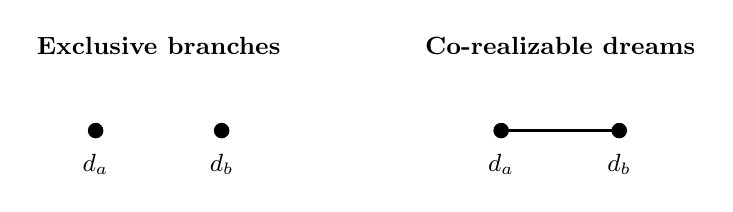
\begin{tikzpicture}[scale=1,every node/.style={font=\small}]
\node[font=\small\bfseries] at (0.8,1.08) {Exclusive branches};
\filldraw[fill=black] (0,0) circle(2.6pt);
\filldraw[fill=black] (1.6,0) circle(2.6pt);
\node[below=5pt] at (0,0) {$d_a$};
\node[below=5pt] at (1.6,0) {$d_b$};
\node[font=\small\bfseries] at (5.9,1.08) {Co-realizable dreams};
\draw[line width=1.1pt] (5.15,0)--(6.65,0);
\filldraw[fill=black] (5.15,0) circle(2.6pt);
\filldraw[fill=black] (6.65,0) circle(2.6pt);
\node[below=5pt] at (5.15,0) {$d_a$};
\node[below=5pt] at (6.65,0) {$d_b$};
\end{tikzpicture}
\caption{Both conditions have $\Dream=\{d_a,d_b\}$ and identical literal MUSIC. Only the right-hand realizability complex has the $1$-simplex $\{d_a,d_b\}$. This is a compatibility diagram, not a metric or a claim about measured performance.}
\label{fig:compat}
\end{figure}

Higher-dimensional faces record collections of three or more dreams that can occur in one run. Crucially, pairwise compatibility does not guarantee triple compatibility. Thus the complex can contain all three edges of a triangle but not its filled two-dimensional face. This illustrates why generalized cooperation cannot be reduced merely to checking pairs of dreams.


\begin{example}[Pairwise compatibility need not imply triple compatibility]\label{ex:triple}
Let $\Dream_c=\{a,b,c\}$ and let the maximal occurrence sets of legal runs be
$\mathsf E(\rho_1)=\{a,b\}$, $\mathsf E(\rho_2)=\{a,c\}$, and
$\mathsf E(\rho_3)=\{b,c\}$. The coverage assumption holds. Every pair of
vertices is a face of $K_c$, while $\{a,b,c\}\notin K_c$: no run witnesses the triple.
Thus a filled triangle is not implied by its three edges. This construction is an
abstract legal-run example, not a claim about a fixed GBG+ scheduler.
\end{example}

\begin{proposition}[Unrestricted finite-complex representation]\label{prop:finite-realization}
Every abstract simplicial complex $L$ on a finite vertex set $D$ with
$\bigcup L=D$ is the finite realizability complex of an abstract run model
with possible-dream set $D$. This assertion need not survive imposed locality,
fairness, or transition-system restrictions.
\end{proposition}
\begin{proof}
For each inclusion-maximal face $F$ of $L$, introduce a legal run whose
dream-occurrence set is precisely $F$. Finiteness ensures every face is
contained in a maximal face. Hence the subsets of occurrence sets are exactly
$L$, and coverage holds. If $D=\varnothing$, use a single run with empty
occurrence set and the complex $\{\varnothing\}$.
\end{proof}

\paragraph{Relation to prior art.} Using simplicial complexes to encode permitted joint states and behavior has a substantial history in distributed computing, including Herlihy--Shavit \cite{herlihy-shavit} and Herlihy--Kozlov--Rajsbaum \cite{herlihy-kozlov}. Our elementary complex construction is a model-specific adaptation of standard mathematics; its definition alone does not warrant an originality claim.

\section{Theorems, theory extension, and the certified BANK}
The word \emph{theory} has two relevant meanings. The \emph{object theory} $\Gamma$ determines which mathematical formulas follow from premises. The \emph{metatheory} describes ATP states, BANKs, possible game histories, and sets of dreams. MUSIC belongs naturally to the latter unless the object language itself is enriched to talk about game states and report sets.

\begin{proposition}[Conservative introduction as notation]\label{prop:defextend}
In an ambient set theory with the needed report and history sets, introducing the symbol $\Music(c)$ by \eqref{eq:music} is a definitional extension: each occurrence may be eliminated in favor of $\PSet(\Dream_c)$. Consequently, this act of naming MUSIC creates no new theorems in the previously available language.
\end{proposition}
\begin{proof}
Replace every new occurrence of $X\in\Music(c)$ with $X\subseteq\Dream_c$ and every instance of $\Music(c)$ with its uniquely defined existing set. The translation eliminates the symbol without adding an independent axiom.
\end{proof}

\begin{remark}[Expressibility is not automatic]
If the object system lacks higher-order quantification, powersets, or a coding of legal episodes, it may not be possible to define MUSIC \emph{internally} using only that system's original vocabulary. It can still be defined in a suitable external set-theoretic metatheory. The assertion ``already in the theory'' must therefore specify the formal language. Likewise, when legality is an informal rule rather than a formal predicate, a fully internal definition requires that missing formalization first.
\end{remark}

\begin{theorem}[Verifier-gated conservativity of MUSIC-guided discovery]\label{thm:bank}
Fix a background theory $\Sigma_0$ with consequence operator $\Cn$ that is extensive, monotone, and idempotent. Let $B_t^{\rm obj}$ be the object-level formulas in a certified BANK after $t$ admissions, with $B_0^{\rm obj}\subseteq\Cn(\Sigma_0)$. Assume that every later admitted object formula is independently verified as a consequence of $\Sigma_0$, with all imported dependencies and undischarged assumptions checked in the same authorized theory context. Search suggestions, including those taken from MUSIC, are not admitted by themselves. Then for every finite $t$,
\begin{equation}\label{eq:bank}
 B_t^{\rm obj}\subseteq\Cn(\Sigma_0),\qquad
 \Cn(\Sigma_0\cup B_t^{\rm obj})=\Cn(\Sigma_0).
\end{equation}
\end{theorem}
\begin{proof}
Induct on the number of deposits. The base case follows from the hypothesis on $B_0^{\rm obj}$. An additional accepted formula is a checked consequence of $\Sigma_0$ under exactly the stipulated dependency contract; the induction property remains true. Hence $\Sigma_0\subseteq\Sigma_0\cup B_t^{\rm obj}\subseteq\Cn(\Sigma_0)$, and monotonicity and idempotence give the equality of consequence closures. MUSIC can affect candidate selection but is not a premise-injecting rule.
\end{proof}

This result deliberately parallels conservativity arguments in the five-ATP dreaming manuscript \cite{tenneson-dreaming} and the later AMLD+0 monograph \cite{tenneson-wcf}. Independently checkable proof certificates are a general objective in automated reasoning \cite{certificate}; this manuscript assumes the check succeeds and does not assert an actual checker run. It does \emph{not} assume that every piece of historical or operational knowledge is a formula in the same object language. Nor does it cover a changed axiom base, new external oracle facts, an unsound checker, or unverified imports. Such cases require separate treatment rather than being called conservative by definition.

\begin{corollary}[No theoremhood advantage from the name MUSIC]
Under \cref{thm:bank}, adding MUSIC-guided candidate generation can change the sequence and cost of verified discoveries, but not the object-theoretic consequence set $\Cn(\Sigma_0)$.
\end{corollary}

\section{Why MUSIC does not automatically produce proof speedup}
Three claims must be kept separate:
\begin{enumerate}
\item \emph{Existence:} $\Music(c)$ is mathematically definable.
\item \emph{Representational adequacy:} a score or report union preserves the particular property the ATP needs (\cref{thm:factor}).
\item \emph{Operational advantage:} the representation improves the total cost or success probability of an implemented search process, against a declared competitor.
\end{enumerate}
The first is elementary under set assumptions; the second is conditional on what reports preserve; the third is an empirical and algorithmic research question.

For an experiment, an honest cost ledger should at least include
\begin{equation}\label{eq:cost}
 C_{\rm total}=C_{\rm search}+C_{\rm dream}+C_{\rm encode}
 +C_{\rm retrieve}+C_{\rm verify}+C_{\rm store}
 +C_{\rm communicate}+C_{\rm schedule}+C_{\rm restart}.
\end{equation}
The exact categories and weights must be frozen before comparison. This follows the full-accounting concern in \cite{tenneson-wcf}: cached or compressed evidence has acquisition, verification, and handling costs. Mathematical cardinality supplies no upper bound on practical storage or enumeration resources.

\begin{proposition}[No architecture-independent strict advantage]\label{prop:noall}
No fixed MUSIC-guided algorithm can be strictly faster than \emph{every} competing algorithm on every input under a common deterministic cost convention, if the competitor class permits an exact implementation of that same algorithm.
\end{proposition}
\begin{proof}
Choose the competitor to implement the identical algorithm with the identical resource accounting. Its cost on each input is equal, contradicting the demanded strict inequality.
\end{proof}
This very simple obstruction matters: MUSIC cannot establish universal dominance merely by being a larger combinatorial structure. A real research claim should specify what is measured and what information competing procedures receive.

\begin{example}[An honest positive control]
Suppose a dream reports a verified recurring proof-search motif, and a guided solver uses it to propose a successful next candidate before an otherwise fixed enumeration order would reach that candidate. This can yield fewer candidate checks on that input, with exactly the same final verifier. It demonstrates \emph{possible local guidance}; it does not show that the motif could not have been learned or represented without MUSIC, that net cost decreased after overhead, or that a general proof family has been accelerated. These further claims require controls.
\end{example}

\section{A research protocol for distinguishing the constructions}
The definitional framework suggests a reproducible experiment without assuming a pre-existing persistent dream runtime.
\begin{enumerate}[label=\textbf{E\arabic*.}]
\item \textbf{Freeze the formal interface.} Specify the logic, initial BANK and theory fingerprint, the full state $s$, legal $\mathbb Z^2$ move rules, internal player roster, scheduler, and certificate schema. Do not identify five federation ATPs with the internal player count.
\item \textbf{Choose an observable report scheme.} Compare (i) untagged visited locations, (ii) time- and actor-tagged reports, and (iii) full provenance-linked reports. Record which history properties factor through each observation map.
\item \textbf{Enumerate a bounded instance.} For a small time horizon, compute $\Dream_c$, literal $\Music(c)$ when finite, and the faces of $K_c$. The full powerset is not necessary for large instances; store $\Dream_c$ and an appropriate representation of legal joint realizability.
\item \textbf{Test preservation.} For every pair of distinct histories sharing a dream union, compare terminal labels, checker receipts, dependency scope, and cost. A disagreement falsifies recoverability of that field for the proposed report format.
\item \textbf{Test discovery without certificate laundering.} Compare MUSIC-guided selection against identical search with random, unmusical set, and ordinary proof-reuse representations. Only the independent verifier may admit results to BANK.
\item \textbf{Count all costs and ablate components.} Include the encoder, pattern extractor, scheduler, storage, reconstruction, and failed verifier calls. Report matched budgets, seed choices, censored runs, and counterexamples. A musical name is not an advantage until a measurable effect is established.
\end{enumerate}

\paragraph{Candidate for distinctiveness, not a priority claim.} Treating $\Music(c)=\PSet(\Dream_c)$ as an explicit coordinate of ATP reflective possibility, then refining it to the execution-sensitive complex $K_c$ under the author's BANK/GBG+ architecture, is a candidate research synthesis. The powerset laws, factorization criterion, and simplicial closure are standard mathematical consequences. No comprehensive novelty search or independently checked new theorem certificate is claimed here.

\section{A comparison with nearby mathematical concepts}
\begin{table}[htbp]
\centering\small
\renewcommand{\arraystretch}{1.18}
\begin{tabularx}{\textwidth}{@{}p{.21\textwidth}X X@{}}
\toprule
Object & What it retains & What it can forget \\
\midrule
History $h$ & Ordered legal events, if completely recorded & Nothing by design, but recording may be partial \\
Dream $d(h)$ & Union of location reports & Order, multiplicity, authority, if absent from report tags \\
Possible dreams $\Dream_c$ & Which report unions can occur individually & Which dreams coexist during one execution \\
Literal $\Music(c)$ & Every subset of $\Dream_c$ & The same joint-realizability information; its content is fixed by $\Dream_c$ \\
Joint $\JMusic(c)$ & All jointly occurring dream collections & Temporal ordering within a witnessing run \\
Finite complex $K_c$ & Finite joint-compatibility faces & Infinite co-realizability not determined by finite faces without extra hypotheses \\
Certified BANK & Admitted claims and verification provenance & Unverified paths that might have been explored \\
\bottomrule
\end{tabularx}
\caption{Different abstractions answer different questions. A report format with complete tags can preserve more than an untagged location union; it is not automatically an equivalent full operational trace.}
\end{table}

The full family $\JMusic(c)$ may include infinite collections, whereas $K_c$ records only \emph{finite} jointly realizable subsets. The following explicit example shows that the passage from finite to infinite co-realizability is not valid without an additional compactness hypothesis.


\begin{proposition}[Finite faces do not determine infinite co-realizability]\label{prop:infinite-gap}
There are two abstract run models with identical countably infinite dream space
$D$, identical finite realizability complex $K=\Fin(D)$, and different full
joint families $\JMusic$.
\end{proposition}
\begin{proof}
Take $D=\{d_0,d_1,\ldots\}$. In the first model, permit a run with
occurrence set $F$ for every \emph{finite} $F\subseteq D$, and no other runs.
Then $\JMusic(c_1)=\Fin(D)$. In the second, keep those runs and also permit
one run with occurrence set $D$. Then $\JMusic(c_2)=\PSet(D)$.
Both models cover $D$ and have $K_1=K_2=\Fin(D)$, but
$D\notin\JMusic(c_1)$ and $D\in\JMusic(c_2)$.
\end{proof}

\section{Open problems}
\begin{enumerate}[label=\textbf{O\arabic*.}]
\item \textbf{Invariant preservation.} Characterize the smallest tags and certificate references for which settlement status, provenance, and relevant resource cost factor through the report-union map.
\item \textbf{Cooperation topology.} Determine which classes of abstract simplicial complexes arise as $K_c$ for specified locally finite GBG+ transition systems and fair schedules. The unrestricted representation result (Proposition~\ref{prop:finite-realization}) shows why such restrictions are essential. Identify which topological features correspond to real obligations rather than an arbitrary encoding.
\item \textbf{Temporal enrichment.} Construct a sequence-sensitive or event-structure enrichment that distinguishes different orders of the same jointly realizable dream collection while retaining the user's union-of-reports definition for each individual dream.
\item \textbf{Minimal representation.} Determine when a quotient preserving settlement-relevant observations is strictly smaller than a full event log \emph{after} authentication and reconstruction costs are charged.
\item \textbf{Operational discovery.} On preregistered conjecture suites, test whether structure derived from $K_c$ or a richer score improves certified discoveries per total unit cost over strong nonmusical controls.
\item \textbf{Formalization boundary.} Give an explicit translation from the external set-theoretic definitions into the typed history and BANK formalism of a chosen AMLD+0 implementation, and mechanically check the resulting safety theorem.
\end{enumerate}

\section{AMLD+0 settlement report and claim ledger}
\noindent The role labels below are an analytical reporting convention, informed by the accompanying bootstrap description \cite{tenneson-bootstrap}, not a record of separately instantiated Pioneer agents.
\paragraph{Frozen task.} Determine whether the proposed ``set of sets of possible dreams'' is mathematically definable under fixed BANK, players, and starting or intermediate conditions, identify its consequences for definitions, theorems, and object theory, and assess whether the construct was implicit in the existing architecture.

\begin{center}
\small
\renewcommand{\arraystretch}{1.17}
\begin{tabularx}{\textwidth}{@{}p{.13\textwidth}X@{}}
\toprule
Role & Supported result \\
\midrule
\status{P} & Powerset existence and recovery; monotonicity under explicit dream-space inclusion; factorization criterion; realizability-complex theorem; verifier-gated conservativity. \\
\status{R} & Counterexamples to order recovery and to the assertion that individually possible dreams must jointly occur; universal strict-speedup claim fails. \\
\status{D} & Internal expressibility depends on the logic; preservation depends on report tags; speedup depends on cost and baseline. \\
\status{I} & No independence proof is offered; mere incompleteness of search is not evidence of independence. \\
\status{C} & No inconsistency detected in the stipulated mathematics; no formal consistency proof for a complete ATP implementation is claimed. \\
\bottomrule
\end{tabularx}
\end{center}

\noindent\textbf{Display result: $\status{P}$ for the restricted structural statement.} This is a report about the mathematical propositions established here, not an externally checked AMLD+0 machine receipt. The stronger conjectures about measurable enhancement and genuinely novel mathematical consequences remain open.

\paragraph{Claim classification.} The set-theoretic recovery, cardinality, Boolean algebra, factorization, downward-closure, and abstract complex-realization results are proved in the article and draw on established mathematics. The finite/infinite separation is a constructive counterexample within the stipulated abstract run semantics. The BANK result is conditional on a sound verifier and correct dependency scoping, closely related to the source manuscript's established conservative-growth argument. The proposal to use the names MUSIC and realizability MUSIC inside this particular dreaming architecture is a research definition, not by itself a theorem of mathematical originality. Runtime benefit, full-system installation, and measured discovery advantage have not been established.

\section*{Acknowledgment of source and method}
\addcontentsline{toc}{section}{Acknowledgment of source and method}
The core MUSIC definition, its dependence on BANK/players/conditions, and the definition of dreams as unions of location reports were specified by Brian Tenneson in the research dialogue of November 3, 2026. The formal developments, proofs, criticism, comparative exposition, and manuscript preparation were AI-assisted and directed by that problem formulation. The additional source, \emph{Who Checks the Federation?} 7.10, was supplied by Google Drive link. No claim of machine-checked proofs, authenticated multi-agent execution, or complete prior-art review should be inferred from the prose.

\begin{thebibliography}{9}
\bibitem{tenneson-dreaming}
B. Tenneson, \emph{Dreaming in a Five-ATP Federation: One AMLD+0 Conjecture Settler, Five ATP Members, Certified Dreaming, and Self-Directed Mathematical Study}, research manuscript 0.4R (ATLAS-repaired), October 29, 2026.\newline
\href{https://btenneson.github.io/pub/cs.LO_Logic_in_Computer_Science/five_atp_one_amld_dreaming_0_4r_atlas_repaired/}{Author repository entry}.

\bibitem{tenneson-core}
B. Tenneson, \emph{The Invariant Core and the Geometry of Settlement}, 2026.\newline
\href{https://btenneson.github.io/pub/cs.LO_Logic_in_Computer_Science/invariant_core_geometry_settlement/}{Author repository entry}.

\bibitem{tenneson-wcf}
B. Tenneson, \emph{Who Checks the Federation? Non-Singleton Settlement, Certified Cooperation, and the AMLD+0 Research Program}, Integrated Research Edition 7.10, November 3, 2026; user-provided edition.\newline
\href{https://drive.google.com/file/d/14ud5bXYnV5dfWGsFjF9Byq2uKy--lA-r/view}{User-supplied Google Drive source}.

\bibitem{tenneson-bootstrap}
B. Tenneson, \emph{AMLD+0 Conversational Operations Bootstrap}, user-supplied markdown protocol (November 3, 2026); filename: \path{AMLD0_ChatGPT_Bootstrap_REGEN.md}. \href{https://drive.google.com/file/d/1CQ5Wo-TUMYcIXtmehPUFZ6zd56bDuCjQ/view}{Source file}.

\bibitem{herlihy-shavit}
M. Herlihy and N. Shavit, ``The Topological Structure of Asynchronous Computability,'' \emph{Journal of the ACM} \textbf{46}(6), 858--923 (1999). DOI: \href{https://doi.org/10.1145/331524.331529}{10.1145/331524.331529}.

\bibitem{herlihy-kozlov}
M. Herlihy, D. Kozlov, and S. Rajsbaum, \emph{Distributed Computing Through Combinatorial Topology}, Morgan Kaufmann/Elsevier, first edition (2013; copyright 2014). ISBN 9780124045781. \href{https://shop.elsevier.com/books/distributed-computing-through-combinatorial-topology/herlihy/978-0-12-404578-1}{Publisher record}.

\bibitem{certificate}
H. Barbosa et al., ``Generating and Exploiting Automated Reasoning Proof Certificates,'' \emph{Communications of the ACM} \textbf{66}(10), 86--95 (2023). DOI: \href{https://doi.org/10.1145/3587692}{10.1145/3587692}.
\end{thebibliography}

\clearpage
\thispagestyle{plain}
\vspace*{10mm}
\begin{center}
{\Large\bfseries AI Authorship and Mathematical Reliability Disclaimer}\par
\vspace{4pt}
{\small Final-page statement}
\end{center}
\vspace{8pt}
This manuscript is a hybrid human--AI research exposition. Brian Tenneson supplied the motivating research program, the proposed definition of MUSIC as the set of sets of possible dreams conditioned on the BANK, players, and starting or intermediate state, and the conception of dreams as unions of location reports. ChatGPT (GPT-6), used here as an AI writing and reasoning assistant, developed portions of the formal notation, examples, propositions, proofs, comparisons, bibliography, and editorial organization under human direction. References to AMLD+0 Pioneer roles describe a structured analysis protocol, not independently operating, authenticated agents. The present ``Atlas audit'' denotes an iterative manuscript review and repair by ChatGPT, not an independent formal checker or authenticated multi-agent execution. Names or descriptions of other AI-assisted editorial and audit processes in earlier source works do not imply that those systems audited this manuscript.

\medskip
The exposition aims to be factually accurate, logically coherent, mathematically rigorous, and sufficiently complete in the practical sense of presenting relevant assumptions, definitions, arguments, evidence limitations, and context. Here \emph{complete} does not mean completeness in the technical sense of G\"odel's completeness or incompleteness theorems. Claims described as proved are supported by the arguments written in this manuscript and the explicit assumptions on which they depend. They have not been independently checked by a formal proof assistant or an authenticated external ATP federation. No guarantee is made that every statement is correct, consistent, provable, original, or immune to counterexample or correction. Some claims may be conditional, provisional, or later refutable. Source references and the phrase ``candidate for distinctiveness'' do not establish exhaustive prior-art coverage or priority of discovery.

\medskip
The separation between speculative discovery and accepted mathematical evidence is substantive: neither a dream, a MUSIC collection, a model-generated argument, nor a narrative of verification constitutes an externally checked proof certificate. Readers should independently inspect assumptions and derivations, verify bibliographic details as needed, and withhold any claim of implemented or externally certified capability unless supporting artifacts are actually available. This statement intentionally appears as the last page of the document.

\vfill
\begin{center}\small\itshape End of manuscript\end{center}
\end{document}